% !TeX program = xelatex
\documentclass[a4paper,10pt]{article}

% ============================================================================
% កញ្ចប់កិច្ចតែងការបង្រៀនគណិតវិទ្យាថ្នាក់ទី៨ (៥០ នាទី - គំរូ 5Es - គ្មានស្លាយ LCD)
% មេរៀនទី១៤ ៖ ផ្ទៃក្រឡាពហុកោណ — ចំណុច ២. ផ្ទៃក្រឡាចតុកោណស្មើ (AREA2)
% វិធីសាស្ត្រ៖ Enclosing-Rectangle 8-Triangle Symmetry Frame & Backward-Faded Examples
% ============================================================================
\usepackage[a4paper, left=0.95cm, right=0.95cm, top=0.85cm, bottom=0.92cm, footskip=0.52cm]{geometry}
\usepackage{amsmath, amssymb}
\usepackage{unicode-math}
\usepackage{fontspec}
\usepackage{longtable, array, multirow, colortbl}
\usepackage[table]{xcolor}
\usepackage{enumitem}
\usepackage{pifont}
\usepackage{fancyhdr}
\usepackage{tikz}
\usetikzlibrary{calc, arrows.meta, angles, quotes, decorations.markings, positioning, babel}

\makeatletter
\let\@expl@@@mark@update@singlecol@structures@@\relax
\makeatother

% ============================================================================
% ការកំណត់ពុម្ពអក្សរផ្លូវការ (Cross-Platform Windows Local + Cloud fonts/)
% ============================================================================
\providecommand{\NGSFindFonts}{%
  \IfFileExists{C:/Windows/Fonts/cambria.ttc}{%
    \def\NGSSysPath{C:/Windows/Fonts/}%
    \def\NGSUserPath{C:/Users/KIT/AppData/Local/Microsoft/Windows/Fonts/}%
  }{%
    \IfFileExists{./fonts/KhmerOSsiemreap.ttf}{\def\NGSSysPath{./fonts/}\def\NGSUserPath{./fonts/}}{%
    \IfFileExists{../fonts/KhmerOSsiemreap.ttf}{\def\NGSSysPath{../fonts/}\def\NGSUserPath{../fonts/}}{%
    \IfFileExists{../../fonts/KhmerOSsiemreap.ttf}{\def\NGSSysPath{../../fonts/}\def\NGSUserPath{../../fonts/}}{%
    \IfFileExists{../../../fonts/KhmerOSsiemreap.ttf}{\def\NGSSysPath{../../../fonts/}\def\NGSUserPath{../../../fonts/}}{%
    \IfFileExists{../../../../fonts/KhmerOSsiemreap.ttf}{\def\NGSSysPath{../../../../fonts/}\def\NGSUserPath{../../../../fonts/}}{%
    \IfFileExists{../../../../../fonts/KhmerOSsiemreap.ttf}{\def\NGSSysPath{../../../../../fonts/}\def\NGSUserPath{../../../../../fonts/}}{%
    \IfFileExists{../../../../../../fonts/KhmerOSsiemreap.ttf}{\def\NGSSysPath{../../../../../../fonts/}\def\NGSUserPath{../../../../../../fonts/}}{%
      \def\NGSSysPath{../../../../../../../fonts/}\def\NGSUserPath{../../../../../../../fonts/}%
    }}}}}}}%
  }%
}
\NGSFindFonts

\setmathfont[Path={\NGSSysPath}, FontIndex=1, Scale=1.02]{cambria.ttc}
\defaultfontfeatures{Ligatures=TeX}

\setmainfont[
  Path={\NGSUserPath},
  Extension=.ttf,
  Script=Khmer,
  BoldFont={KhmerOSsiemreap},
  BoldFeatures={FakeBold=1.8},
  ItalicFont={KhmerOSsiemreap},
  ItalicFeatures={FakeSlant=0.25},
  BoldItalicFont={KhmerOSsiemreap},
  BoldItalicFeatures={FakeBold=1.8, FakeSlant=0.25}
]{KhmerOSsiemreap}

\newfontfamily\muol[Path={\NGSUserPath}, Extension=.ttf, Script=Khmer]{KhmerOSmuollight}
\newfontfamily\NagaBold[Path={\NGSUserPath}, Extension=.ttf]{AKbalthom Naga Bold}
\newfontfamily\Tacteing[Path={\NGSUserPath}, Extension=.TTF]{TACTENG}
\newfontfamily\TimesEn[Path={\NGSSysPath}, Extension=.ttf, BoldFont={timesbd}, ItalicFont={timesi}, BoldItalicFont={timesbi}]{times}
\newfontfamily\CalibriFont[Path={\NGSSysPath}, Extension=.ttf]{calibri}
\newfontfamily\CourierNew[Path={\NGSSysPath}, Extension=.ttf]{cour}

\newcommand{\wcirc}{{\CourierNew\selectfont o}}

\XeTeXlinebreaklocale "km"
\XeTeXlinebreakskip = 0pt plus 1pt minus 0.1pt

% ============================================================================
% ពណ៌ផ្លូវការតាមគំរូ ls_plan.tex
% ============================================================================
\definecolor{headgray}{HTML}{D9D9D9}
\definecolor{stepgray}{HTML}{BFBFBF}
\definecolor{red5e}{HTML}{C00000}
\definecolor{darkred}{HTML}{800000}

\pagestyle{fancy}
\fancyhf{}
\renewcommand{\headrulewidth}{0pt}
\fancyfoot[R]{{\CalibriFont\fontsize{9.5pt}{11pt}\selectfont\thepage}}

\setlength{\parindent}{0pt}
\setlength{\parskip}{0pt}
\setlength{\LTpre}{2pt}
\setlength{\LTpost}{2pt}
\setlength{\tabcolsep}{4.5pt}
\arrayrulewidth=0.4pt

\newcolumntype{L}[1]{>{\raggedright\arraybackslash}p{#1}}

% ============================================================================
% ម៉ាក្រូជំនួយ (Helper Macros)
% ============================================================================
\newcommand{\en}[1]{{\TimesEn #1}}
\newcommand{\enbf}[1]{{\TimesEn\textbf{#1}}}
\newcommand{\unit}[1]{\,\text{\en{#1}}}
\newcommand{\fiveE}[1]{{\NagaBold\fontsize{9.5pt}{13pt}\selectfont\textcolor{red5e}{#1}}}
\newcommand{\timenote}[1]{\textcolor{darkred}{\textit{#1}}}
\newcommand{\cnum}[1]{{\fontsize{10.5pt}{12pt}\selectfont\ding{\numexpr181+#1\relax}}\hspace{0.2em}}
\newcommand{\cfig}[1]{\par\vspace{4pt}{\centering #1\par}\vspace{4pt}}
\newcommand{\stepheader}[1]{\multicolumn{3}{|c|}{\cellcolor{stepgray}\muol #1} \\* \noalign{\hrule height 0.4pt}}
\newcommand{\tri}[1]{\ensuremath{\triangle #1}}
\newcommand{\ang}[1]{\ensuremath{\angle #1}}
\newcommand{\cg}{\ensuremath{\cong}}
\newcommand{\khmflourish}{{\Tacteing\fontsize{36pt}{14pt}\selectfont\raisebox{-5pt}{3}}}

\newcommand{\rightbox}[4][0.20cm]{%
  \draw[black, line width=0.8pt]
    ($(#3)!#1!(#2)$) -- ($($(#3)!#1!(#2)$)+($(#3)!#1!(#4)$)-(#3)$) -- ($(#3)!#1!(#4)$);
}

\tikzset{
  tk1/.style={postaction={decorate},decoration={markings,mark=at position 0.50 with {\draw[black, line width=0.85pt](0,-0.095)--(0,0.095);}}},
  tk2/.style={postaction={decorate},decoration={markings,
    mark=at position 0.45 with {\draw[black, line width=0.85pt](0,-0.095)--(0,0.095);},
    mark=at position 0.55 with {\draw[black, line width=0.85pt](0,-0.095)--(0,0.095);}}}
}

% ============================================================================
% ម៉ាក្រូរូបភាព TikZ ស-ខ្មៅ សមាមាត្រច្បាស់ (3.8 cm – 7.2 cm, អក្សរខ្មៅ 100%)
% ============================================================================

% ១. រូបបេសកកម្ម E1៖ ខ្លែងឯកខ្មែររាងចតុកោណស្មើក្នុងក្រដាសចតុកោណកែង 6dm x 8dm
\newcommand{\figEngageAREATwo}{%
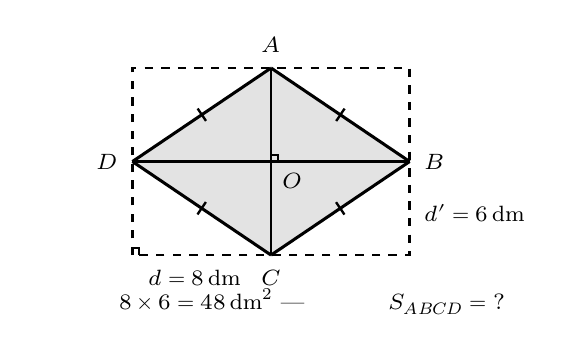
\begin{tikzpicture}[scale=0.44, every node/.style={font=\footnotesize, text=black}]
  \fill[white] (0,0) rectangle (8,5.4);
  \fill[gray!22] (4,0) -- (8,2.7) -- (4,5.4) -- (0,2.7) -- cycle;
  \draw[black, line width=0.9pt, dashed] (0,0) rectangle (8,5.4);
  \draw[black, line width=1.1pt, tk1] (4,0) -- (8,2.7);
  \draw[black, line width=1.1pt, tk1] (8,2.7) -- (4,5.4);
  \draw[black, line width=1.1pt, tk1] (4,5.4) -- (0,2.7);
  \draw[black, line width=1.1pt, tk1] (0,2.7) -- (4,0);
  \draw[black, line width=0.95pt] (0,2.7) -- (8,2.7) (4,0) -- (4,5.4);
  \rightbox[0.20cm]{4,5.4}{4,2.7}{8,2.7}
  \rightbox[0.20cm]{0,5.4}{0,0}{8,0}
  \node[above=2pt] at (4,5.4) {$A$};
  \node[right=2pt] at (8,2.7) {$B$};
  \node[below=2pt] at (4,0) {$C$};
  \node[left=2pt] at (0,2.7) {$D$};
  \node[below right=1pt] at (4,2.7) {$O$};
  \node[below=2pt] at (1.8,0) {$d = 8\unit{dm}$};
  \node[right=2pt] at (8,1.2) {$d' = 6\unit{dm}$};
  \node at (4,-1.35) {ក្រដាសស៊ុមធំ $8\times 6 = 48\unit{dm}^2$ — តើផ្ទៃខ្លែង $S_{ABCD} = ?$};
\end{tikzpicture}}

% ២. រូប E2៖ ស៊ុមចតុកោណកែងបំបែកជាត្រីកោណកែង 8 ប៉ុនគ្នា (4 ប្រផេះក្នុង + 4 សក្រៅ)
\newcommand{\figExploreFrameAREATwo}{%
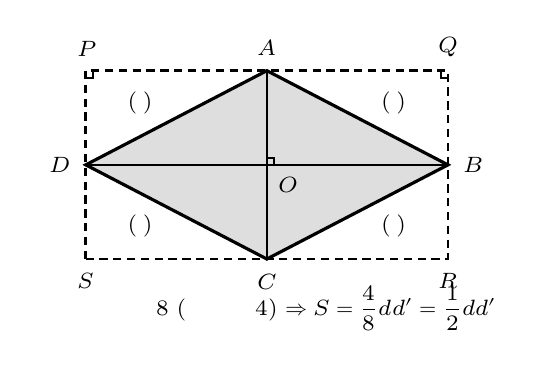
\begin{tikzpicture}[scale=0.46, every node/.style={font=\footnotesize, text=black}]
  \fill[white] (0,0) rectangle (10,5.2);
  \fill[gray!26] (5,0) -- (10,2.6) -- (5,5.2) -- (0,2.6) -- cycle;
  \draw[black, line width=0.95pt, densely dashed] (0,0) rectangle (10,5.2);
  \draw[black, line width=1.15pt] (5,0) -- (10,2.6) -- (5,5.2) -- (0,2.6) -- cycle;
  \draw[black, line width=0.95pt] (0,2.6) -- (10,2.6) (5,0) -- (5,5.2);
  \rightbox[0.20cm]{5,5.2}{5,2.6}{10,2.6}
  \rightbox[0.20cm]{0,2.6}{0,5.2}{5,5.2}
  \rightbox[0.20cm]{5,5.2}{10,5.2}{10,2.6}
  \node[above=1.5pt] at (0,5.2) {$P$};
  \node[above=1.5pt] at (10,5.2) {$Q$};
  \node[below=1.5pt] at (10,0) {$R$};
  \node[below=1.5pt] at (0,0) {$S$};
  \node[above=2pt] at (5,5.2) {$A$};
  \node[right=2pt] at (10,2.6) {$B$};
  \node[below=2pt] at (5,0) {$C$};
  \node[left=2pt] at (0,2.6) {$D$};
  \node[below right=1pt] at (5,2.6) {$O$};
  % លេខសម្គាល់ត្រីកោណទាំង 8
  \node at (3.6,3.4) {១};
  \node at (6.4,3.4) {២};
  \node at (6.4,1.8) {៣};
  \node at (3.6,1.8) {៤};
  \node at (1.5,4.3) {(៥)};
  \node at (8.5,4.3) {(៦)};
  \node at (8.5,0.9) {(៧)};
  \node at (1.5,0.9) {(៨)};
  \node at (5,-1.35) {ត្រីកោណកែងប៉ុនគ្នា $8$ (ក្នុងខ្លែង $4$) $\Rightarrow S = \dfrac{4}{8}dd' = \dfrac{1}{2}dd'$};
\end{tikzpicture}}

% ៣. រូប E3៖ សម្រាយបញ្ជាក់ផ្លូវការតាមសៀវភៅគោល ទំ.១៩០ (ពុះតាមអង្កត់ទ្រូង BD)
\newcommand{\figExplainProofAREATwo}{%
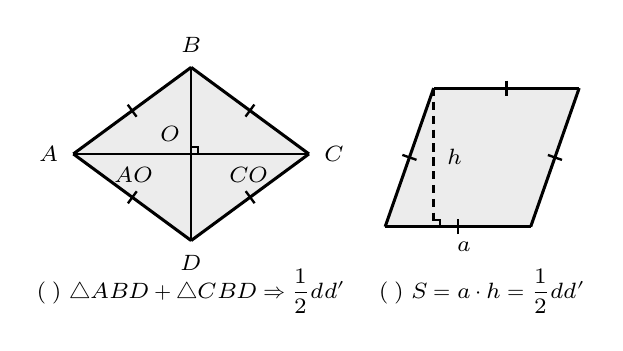
\begin{tikzpicture}[scale=0.44, every node/.style={font=\footnotesize, text=black}]
  \begin{scope}[shift={(0,0)}]
    \coordinate (A) at (0,2.5);
    \coordinate (B) at (3.4,5.0);
    \coordinate (C) at (6.8,2.5);
    \coordinate (D) at (3.4,0);
    \coordinate (O) at (3.4,2.5);
    \fill[gray!15] (A)--(B)--(C)--(D)--cycle;
    \draw[black, line width=1.1pt, tk1] (A)--(B);
    \draw[black, line width=1.1pt, tk1] (B)--(C);
    \draw[black, line width=1.1pt, tk1] (C)--(D);
    \draw[black, line width=1.1pt, tk1] (D)--(A);
    \draw[black, line width=0.95pt] (A)--(C) (B)--(D);
    \rightbox[0.19cm]{B}{O}{C}
    \node[left=2pt] at (A) {$A$};
    \node[above=2pt] at (B) {$B$};
    \node[right=2pt] at (C) {$C$};
    \node[below=2pt] at (D) {$D$};
    \node[above left=1pt] at (O) {$O$};
    \node[below=1pt] at (1.75,2.5) {$AO$};
    \node[below=1pt] at (5.05,2.5) {$CO$};
    \node at (3.4,-1.45) {(១) $\tri{ABD}+\tri{CBD} \Rightarrow \dfrac{1}{2}dd'$};
  \end{scope}
  \begin{scope}[shift={(9.0,0.4)}]
    \coordinate (A) at (0,0);
    \coordinate (B) at (4.2,0);
    \coordinate (C) at (5.6,4.0);
    \coordinate (D) at (1.4,4.0);
    \coordinate (H) at (1.4,0);
    \fill[gray!15] (A)--(B)--(C)--(D)--cycle;
    \draw[black, line width=1.1pt, tk1] (A)--(B);
    \draw[black, line width=1.1pt, tk1] (B)--(C);
    \draw[black, line width=1.1pt, tk1] (C)--(D);
    \draw[black, line width=1.1pt, tk1] (D)--(A);
    \draw[black, line width=0.85pt, densely dashed] (D)--(H);
    \rightbox[0.19cm]{D}{H}{B}
    \node[below=2pt] at (2.3,0) {$a$};
    \node[right=1.5pt] at (1.4,2.0) {$h$};
    \node at (2.8,-1.85) {(២) $S = a\cdot h = \dfrac{1}{2}dd'$};
  \end{scope}
\end{tikzpicture}}

% ៤. រូប E4៖ លំហាត់គំរូទី 1 (d=13, d'=14) និងគំរូទី 2 (S=1000 mm^2, d=10 mm)
\newcommand{\figModelExAREATwo}{%
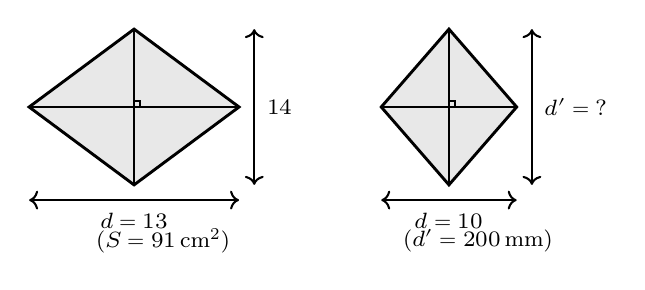
\begin{tikzpicture}[scale=0.43, every node/.style={font=\footnotesize, text=black}]
  \begin{scope}[shift={(0,0)}]
    \coordinate (A) at (0,2.3);
    \coordinate (B) at (3.1,4.6);
    \coordinate (C) at (6.2,2.3);
    \coordinate (D) at (3.1,0);
    \coordinate (O) at (3.1,2.3);
    \fill[gray!18] (A)--(B)--(C)--(D)--cycle;
    \draw[black, line width=1.05pt] (A)--(B)--(C)--(D)--cycle;
    \draw[black, line width=0.9pt] (A)--(C) (B)--(D);
    \rightbox[0.18cm]{B}{O}{C}
    \draw[<->, black, line width=0.75pt] (0,-0.45) -- node[below=1pt] {$d=13$} (6.2,-0.45);
    \draw[<->, black, line width=0.75pt] (6.65,0) -- node[right=1pt] {$14$} (6.65,4.6);
    \node at (3.2,-1.65) {គំរូទី១ ($S=91\unit{cm}^2$)};
  \end{scope}
  \begin{scope}[shift={(9.4,0)}]
    \coordinate (A) at (1.0,2.3);
    \coordinate (B) at (3.0,4.6);
    \coordinate (C) at (5.0,2.3);
    \coordinate (D) at (3.0,0);
    \coordinate (O) at (3.0,2.3);
    \fill[gray!18] (A)--(B)--(C)--(D)--cycle;
    \draw[black, line width=1.05pt] (A)--(B)--(C)--(D)--cycle;
    \draw[black, line width=0.9pt] (A)--(C) (B)--(D);
    \rightbox[0.18cm]{B}{O}{C}
    \draw[<->, black, line width=0.75pt] (1.0,-0.45) -- node[below=1pt] {$d=10$} (5.0,-0.45);
    \draw[<->, black, line width=0.75pt] (5.45,0) -- node[right=1pt] {$d'=?$} (5.45,4.6);
    \node at (3.1,-1.65) {គំរូទី២ ($d'=200\unit{mm}$)};
  \end{scope}
\end{tikzpicture}}

% ៥. រូប E5៖ ប្រតិបត្តិ ទំ.១៩១ (S=120, d=30 => d'=8, a=sqrt(241)) + Exit Check កន្លះអង្កត់ទ្រូង
\newcommand{\figPracticeEvalAREATwo}{%
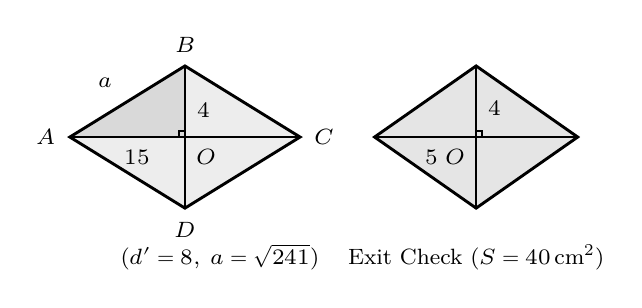
\begin{tikzpicture}[scale=0.43, every node/.style={font=\footnotesize, text=black}]
  \begin{scope}[shift={(0,0)}]
    \coordinate (A) at (0,2.1);
    \coordinate (B) at (3.4,4.2);
    \coordinate (C) at (6.8,2.1);
    \coordinate (D) at (3.4,0);
    \coordinate (O) at (3.4,2.1);
    \fill[gray!14] (A)--(B)--(C)--(D)--cycle;
    \fill[gray!30] (A)--(O)--(B)--cycle;
    \draw[black, line width=1.05pt] (A)--(B)--(C)--(D)--cycle;
    \draw[black, line width=0.9pt] (A)--(C) (B)--(D);
    \rightbox[0.18cm]{B}{O}{A}
    \node[left=1.5pt] at (A) {$A$};
    \node[above=1.5pt] at (B) {$B$};
    \node[right=1.5pt] at (C) {$C$};
    \node[below=1.5pt] at (D) {$D$};
    \node[below right=1pt] at (O) {$O$};
    \node[below=1pt] at (2.0,2.1) {$15$};
    \node[right=1pt] at (3.4,2.9) {$4$};
    \node[above left=1pt] at (1.6,3.2) {$a$};
    \node at (3.4,-1.45) {ប្រតិបត្តិ ($d'=8,\; a=\sqrt{241}$)};
  \end{scope}
  \begin{scope}[shift={(9.0,0)}]
    \coordinate (A) at (0,2.1);
    \coordinate (B) at (3.0,4.2);
    \coordinate (C) at (6.0,2.1);
    \coordinate (D) at (3.0,0);
    \coordinate (O) at (3.0,2.1);
    \fill[gray!20] (A)--(B)--(C)--(D)--cycle;
    \draw[black, line width=1.05pt] (A)--(B)--(C)--(D)--cycle;
    \draw[black, line width=0.9pt] (A)--(C) (B)--(D);
    \rightbox[0.18cm]{B}{O}{C}
    \node[below=1pt] at (1.7,2.1) {$5$};
    \node[right=1pt] at (3.0,2.95) {$4$};
    \node[below left=1pt] at (O) {$O$};
    \node at (3.0,-1.45) {\en{Exit Check} ($S=40\unit{cm}^2$)};
  \end{scope}
\end{tikzpicture}}

% ============================================================================
% ចាប់ផ្ដើមឯកសារ (Document Body)
% ============================================================================
\begin{document}
\fontsize{10pt}{15.2pt}\selectfont

% -------------------- ក្បាលកិច្ចតែងការ (Header) --------------------
\begin{center}
  {\muol\fontsize{11pt}{16pt}\selectfont ព្រះរាជាណាចក្រកម្ពុជា}\\[2pt]
  {\muol\fontsize{10pt}{15pt}\selectfont ជាតិ សាសនា ព្រះមហាក្សត្រ}\\[1pt]
  \khmflourish
\end{center}

\vspace{-26pt}
{\muol\fontsize{9.5pt}{12.8pt}\selectfont
មន្ទីរអប់រំ យុវជន និងកីឡា ខេត្តកំពង់ធំ\\
ការិយាល័យអប់រំ យុវជន និងកីឡា ស្រុកកំពង់ស្វាយ\\
អនុវិទ្យាល័យព្រះក្រសាំង}

\vspace{1pt}
\begin{center}
  {\muol\fontsize{10pt}{14.5pt}\selectfont កិច្ចតែងការបង្រៀន}
\end{center}
\vspace{0pt}

% -------------------- ព័ត៌មានទូទៅ (Metadata) --------------------
{\renewcommand{\arraystretch}{0.98}
\hspace*{4.05cm}%
\begin{tabular}{@{}l l l@{}}
  - \hspace{0.35cm} មុខវិជ្ជា & : & គណិតវិទ្យា ថ្នាក់ទី៨ \\
  - \hspace{0.35cm} ចំណងជើងមេរៀន & : & មេរៀនទី១៤ ផ្ទៃក្រឡាពហុកោណ \\
  - \hspace{0.35cm} ចំណងជើងរង & : & ២. ផ្ទៃក្រឡាចតុកោណស្មើ (ទំព័រ ១៩០--១៩១) \\
  - \hspace{0.35cm} រយៈពេល & : & ១ ម៉ោងសិក្សា (៥០ នាទី) \\
  - \hspace{0.35cm} បង្រៀនដោយ & : & ហុក ប៊ុនថែន \\
  - \hspace{0.35cm} កាលបរិច្ឆេទ & : & ថ្ងៃអង្គារ ទី១៥ ខែធ្នូ ឆ្នាំ២០២៦ \\
\end{tabular}

\vspace{2pt}

% -------------------- I. វត្ថុបំណង --------------------
\textbf{I.} {\muol វត្ថុបំណង}\\[1pt]
\hspace*{0.55cm}%
\begin{tabular}{@{}l l L{14.2cm}@{}}
  \wcirc \hspace{0.25cm} វិជ្ជាសម្បទា & : & សិស្សប្រាប់ទ្រឹស្ដីបទ និងរូបមន្តផ្ទៃក្រឡាចតុកោណស្មើតាមរង្វាស់អង្កត់ទ្រូងទាំងពីរ ($S = \frac{1}{2} d \times d'$) ព្រមទាំងទំនាក់ទំនងជាមួយរូបមន្តប្រលេឡូក្រាម ($S = ah$) បានត្រឹមត្រូវ ។ \\
  \wcirc \hspace{0.25cm} បំណិនសម្បទា & : & សិស្សស្រាយបញ្ជាក់រូបមន្តផ្ទៃក្រឡាចតុកោណស្មើ និងគណនាផ្ទៃក្រឡា រង្វាស់អង្កត់ទ្រូងបាត់ ($d' = \frac{2S}{d}$) និងរង្វាស់ជ្រុងតាមទ្រឹស្ដីបទពីតាករលើសន្លឹកកិច្ចការបានត្រឹមត្រូវ ។ \\
  \wcirc \hspace{0.25cm} ចរិយាសម្បទា & : & សិស្សមានទម្លាប់ពិនិត្យភាពខុសគ្នារវាង «កន្លះអង្កត់ទ្រូង» និង «អង្កត់ទ្រូងពេញ» ព្រមទាំងពិភាក្សាផ្ទៀងផ្ទាត់ហេតុផលគណិតវិទ្យាដោយម៉ត់ចត់ ។ \\
\end{tabular}

\vspace{2pt}

% -------------------- II. សម្ភារៈឧបទេស --------------------
\textbf{II.} {\muol សម្ភារៈឧបទេស}\\[1pt]
\hspace*{0.55cm}\parbox[t]{18.2cm}{$\bullet$ \hspace{0.25cm} សម្រាប់គ្រូ៖ សៀវភៅសិក្សាគោលគណិតវិទ្យាថ្នាក់ទី៨ (ទំ.១៩០--១៩១ និង ១៩៤--១៩៥) ក្ដារខៀន ដីស បន្ទាត់វែង និងសន្លឹកកិច្ចការគំរូ (គ្មានស្លាយ \en{LCD}) ។\\
$\bullet$ \hspace{0.25cm} សម្រាប់សិស្ស៖ សន្លឹកកិច្ចការសិស្ស ស-ខ្មៅ (\en{Worksheet\_AREA2} ២ ទំព័រពេញ) សៀវភៅសិក្សាគោល សៀវភៅសរសេរ បន្ទាត់ក្រិត និងប៊ិច/ខ្មៅដៃ ។}

\vspace{2pt}

% -------------------- III. វិធីសាស្រ្តបង្រៀន --------------------
\textbf{III.} {\muol វិធីសាស្រ្តបង្រៀន}\\[1pt]
\hspace*{0.45cm}%
\begin{tabular}{@{}l l L{14.85cm}@{}}
  $\bullet$ \hspace{0.25cm} គោលវិធី & : & សិស្សមជ្ឈមណ្ឌល (បង្រៀនដោយមិនប្រើស្លាយ \en{LCD} យកសន្លឹកកិច្ចការបំពេញចន្លោះជាគោល) \\
  $\bullet$ \hspace{0.25cm} យុទ្ធវិធីបង្រៀន & : & ស្ថាបនានិយម គំរូ \en{5Es} រួមផ្សំវិធីស៊ុមចតុកោណកែងព័ទ្ធជុំវិញបំបែកត្រីកោណកែង ៨ (\en{Enclosing-Rectangle Symmetry Frame}) និងលំហាត់គំរូថយជំនួយ (\en{Backward-Faded Examples}) \\
\end{tabular}
}

\vspace{2pt}

% -------------------- IV. ដំណើរការបង្រៀន --------------------
\textbf{IV.} {\muol ដំណើរការបង្រៀន}

\vspace{1pt}

\renewcommand{\arraystretch}{1.15}
\begin{longtable}{|L{5.50cm}|L{7.90cm}|L{4.80cm}|}
\hline
\rowcolor{headgray}
\multicolumn{1}{|c|}{\muol សកម្មភាពគ្រូ} &
\multicolumn{1}{c|}{\muol ខ្លឹមសារមេរៀន} &
\multicolumn{1}{c|}{\muol សកម្មភាពសិស្ស} \\
\hline
\endfirsthead

\hline
\rowcolor{headgray}
\multicolumn{1}{|c|}{\muol សកម្មភាពគ្រូ} &
\multicolumn{1}{c|}{\muol ខ្លឹមសារមេរៀន} &
\multicolumn{1}{c|}{\muol សកម្មភាពសិស្ស} \\
\hline
\endhead

\hline
\endfoot

\hline
\endlastfoot

% ==================== ជំហានទី១ (2min) ====================
\stepheader{ជំហានទី១ ៖ រដ្ឋបាលថ្នាក់ (២ នាទី)}
$\bullet$ ពិនិត្យអវត្តមាន សណ្ដាប់ធ្នាប់ និងអនាម័យថ្នាក់រៀន\par\vspace{2pt}
$\bullet$ ចែកសន្លឹកកិច្ចការ \en{Worksheet\_AREA2} (១ សន្លឹកសងខាង) ដល់សិស្សគ្រប់គ្នា
&
$\bullet$ ពិនិត្យវត្តមាន និងការត្រៀមសម្ភារៈសិក្សា (សន្លឹកកិច្ចការ សៀវភៅសិក្សាគោល និងបន្ទាត់ក្រិត)
&
$\circ$ ប្រធានថ្នាក់រាយការណ៍អវត្តមាន\par\vspace{2pt}
$\circ$ ទទួលសន្លឹកកិច្ចការ និងសរសេរឈ្មោះ \\[3pt]
\hline

% ==================== ជំហានទី២ (9min: ≤3 + 3 + E1 3) ====================
\stepheader{ជំហានទី២ ៖ កែកិច្ចការផ្ទះ រំលឹកមេរៀនចាស់ និងភ្ជាប់មេរៀនថ្មី (៩ នាទី)}
\timenote{(កែកិច្ចការផ្ទះ $\le 3\unit{min}$)}\par\vspace{1pt}
$\bullet$ ហៅសិស្ស ២ នាក់ឡើងសរសេរចម្លើយលំហាត់ទី១ និងទី២(រូបទី១) ទំ.១៩៤ លើក្ដារខៀន រួចផ្ទៀងផ្ទាត់រហ័ស
&
\textbf{កំណែកិច្ចការផ្ទះ (ទំ.១៩៤)៖}\par\vspace{1pt}
១. \textbf{លំហាត់ទី១៖} (ក) $S = 12\times 7 = 84\unit{cm}^2$ ; (ខ) $b = 42\div 6 = 7\unit{cm}$ ; (គ) $h = 42.9\div 7.8 = 5.5\unit{cm}$ ។\par\vspace{1pt}
២. \textbf{លំហាត់ទី២(រូបទី១)៖} $S_{SRQP} = 28\times 7 = 196\unit{cm}^2$ និង $8\times x = 196 \Rightarrow x = 24.5\unit{cm}$ ($PR \perp RQ$) ។
&
$\circ$ សិស្ស ២ នាក់ឡើងបំពេញចម្លើយ\par\vspace{1pt}
$\circ$ ផ្ទៀងផ្ទាត់កិច្ចការផ្ទះក្នុងសៀវភៅ \\[3pt]

\timenote{(រំលឹកមេរៀនទាក់ទង $3\unit{min}$)} $\bullet$ សំណួរទី១៖ «តើចតុកោណស្មើមាននិយមន័យដូចម្ដេច?»
&
\textbf{ចំណេះដឹងមូលដ្ឋានភ្ជាប់មេរៀនថ្មី៖} ១. ចតុកោណស្មើជាប្រលេឡូក្រាមដែលមានជ្រុងទាំង ៤ ប៉ុនគ្នា ($AB=BC=CD=DA$) ។
&
$\circ$ ឆ្លើយ៖ «ជាប្រលេឡូក្រាមមានជ្រុងទាំង ៤ ប៉ុនគ្នា» \\[3pt]

\hspace*{0.3em}-- សំណួរទី២៖ «តើអង្កត់ទ្រូងទាំងពីរនៃចតុកោណស្មើមានលក្ខណៈពិសេសអ្វីត្រង់ចំណុចប្រសព្វ $O$?»
&
២. អង្កត់ទ្រូងចតុកោណស្មើកាត់គ្នាកែងត្រង់ចំណុចកណ្ដាលរៀងៗខ្លួន៖ $AC \perp BD$, $OA = OC = \frac{1}{2}AC$ និង $OB = OD = \frac{1}{2}BD$ ។
&
$\circ$ ឆ្លើយ៖ «កែងគ្នា និងចែកគ្នាជាពីរស្មើៗគ្នា» \\[3pt]

\hspace*{0.3em}-- សំណួរទី៣៖ «តើផ្ទៃក្រឡាត្រីកោណមានបាត $b$ និងកម្ពស់កែង $h$ ស្មើនឹងអ្វី?»
&
៣. ផ្ទៃក្រឡាត្រីកោណ៖ $S_{\tri{}} = \dfrac{1}{2} b \times h$ ។
&
$\circ$ ឆ្លើយ៖ «$S = \frac{1}{2}bh$» \\[3pt]

\fiveE{E1 - Engage} \timenote{(3 min)}\par\vspace{1pt}
$\bullet$ ឱ្យសិស្សអានស្ថានភាព \textbf{ផ្នែកទី១} លើសន្លឹកកិច្ចការ (បេសកកម្មពាសក្រដាសខ្លែងឯកខ្មែរ)
&
\textbf{បេសកកម្ម E1៖ ក្រដាសពាសតួខ្លែងឯកខ្មែរ}\par\vspace{1pt}
$\bullet$ ឆ្អឹងឫស្សីខ្វែងកែងគ្នា៖ $AC = d' = 6\unit{dm}$ និង $BD = d = 8\unit{dm}$ ។\par\vspace{1pt}
$\bullet$ ក្រដាសចតុកោណកែងធំ៖ $S_{\text{ក្រដាស}} = 8 \times 6 = 48\unit{dm}^2$ ។
&
$\circ$ អានស្ថានភាពនិងពិនិត្យរូបខ្លែងលើសន្លឹកកិច្ចការ \\[3pt]

\hspace*{0.3em}-- សំណួរ៖ «តើក្រដាសដែលពាសជាប់លើតួខ្លែងរាងចតុកោណស្មើ ស្មើនឹង $48\unit{dm}^2$ ឬ $36\unit{dm}^2$ ឬ $24\unit{dm}^2$?»
&
$\bullet$ សំណួរគន្លឹះ៖ តើផ្ទៃខ្លែង $S_{ABCD}$ ស្មើប៉ុន្មានភាគនៃផ្ទៃក្រដាសចតុកោណកែង $48\unit{dm}^2$? (ទុកផ្ទៀងនៅ E5)
&
$\circ$ គូសធីក $\square$ ទស្សន៍ទាយមុនរៀនលើសន្លឹកកិច្ចការ \\[3pt]

& \cfig{\figEngageAREATwo} & \\[3pt]
\hline

% ==================== ជំហានទី៣ (17min: E2 11 + E3 6) ====================
\stepheader{ជំហានទី៣ ៖ មេរៀនថ្មី — ២. ផ្ទៃក្រឡាចតុកោណស្មើ (១៧ នាទី)}
\fiveE{E2 - Explore} \timenote{(11 min)}\par\vspace{1pt}
$\bullet$ ណែនាំសិស្សធ្វើការជាដៃគូលើ \textbf{ផ្នែកទី២ នៃសន្លឹកកិច្ចការ} (ស៊ុមចតុកោណកែង $PQRS$ ព័ទ្ធជុំវិញចតុកោណស្មើ $ABCD$)
&
\textbf{សកម្មភាពរុករកតាមស៊ុមចតុកោណកែងបំបែកត្រីកោណកែង ៨៖}\par\vspace{1pt}
$\bullet$ ស៊ុមចតុកោណកែង $PQRS$ មានបណ្ដោយ $PQ = BD = d$ និងទទឹង $PS = AC = d'$ នាំឱ្យ $S_{PQRS} = d \times d'$ ។
&
$\circ$ ពិភាក្សាជាដៃគូលើសន្លឹកកិច្ចការ \\[3pt]

$\bullet$ ឱ្យសិស្សរាប់ចំនួនត្រីកោណកែងតូចៗក្នុងចតុកោណស្មើ (ប្រផេះ ១--៤) ធៀបនឹងក្រៅចតុកោណស្មើ (ស ៥--៨)
&
$\bullet$ អង្កត់ទ្រូងកែងគ្នា $AC \perp BD$ ចែកស៊ុម $PQRS$ ជាត្រីកោណកែងតូចៗប៉ុនគ្នាចំនួន $8$ (ក្នុងចតុកោណស្មើមាន $4$ ផ្នែក និងសល់តាមកែងស៊ុម $4$ ផ្នែក) ។\par\vspace{1pt}
$\bullet$ ដូចនេះ $S_{ABCD} = \dfrac{4}{8} S_{PQRS} = \dfrac{1}{2} d \times d'$ ។
&
$\circ$ សម្គាល់ត្រីកោណប៉ុនគ្នាទាំង ៨ និងទាញបានថាផ្ទៃចតុកោណស្មើស្មើពាក់កណ្ដាលផ្ទៃស៊ុម \\[3pt]

& \cfig{\figExploreFrameAREATwo} & \\[3pt]

$\bullet$ ចោទសួរសំណួរអន្ទាក់ការយល់ច្រឡំ ២ ចំណុច៖\par\vspace{1pt}
\hspace*{0.3em}-- ទី១៖ «បើគេយក $S = d \times d'$ ដោយភ្លេចចែកនឹង $2$ តើគេកំពុងគណនាផ្ទៃអ្វី?»
&
\textbf{ការបំបែកអន្ទាក់ការយល់ច្រឡំ៖}\par\vspace{1pt}
$\bullet$ បើគណនា $d \times d'$ គឺជាផ្ទៃក្រឡា \textbf{ស៊ុមចតុកោណកែងធំ $PQRS$} ដែលធំជាងចតុកោណស្មើ ២ ដង!
&
$\circ$ ឆ្លើយ៖ «ជាផ្ទៃស៊ុមចតុកោណកែងធំ មិនមែនផ្ទៃចតុកោណស្មើទេ!» \\[3pt]

\hspace*{0.3em}-- ទី២៖ «បើរូបភាពប្រាប់ $OA = 5\unit{cm}$ និង $OB = 4\unit{cm}$ តើយើងជំនួស $d=5, d'=4$ បានដែរឬទេ?»
&
$\bullet$ $OA$ និង $OB$ ជា \textbf{កន្លះអង្កត់ទ្រូង}ប៉ុណ្ណោះ! ត្រូវគុណនឹង $2$ រកអង្កត់ទ្រូងពេញជាមុន៖ $d = 2(5) = 10\unit{cm}$ និង $d' = 2(4) = 8\unit{cm}$ ។
&
$\circ$ បកស្រាយ៖ «មិនបានទេ ព្រោះ $d, d'$ ជាអង្កត់ទ្រូងពេញ!» \\[3pt]

\fiveE{E3 - Explain} \timenote{(6 min)}\par\vspace{1pt}
$\bullet$ ហៅតំណាងដៃគូសង្ខេបរូបមន្ត រួចគ្រូសរសេរទ្រឹស្ដីបទ និងសម្រាយបញ្ជាក់ពិជគណិតផ្លូវការតាមសៀវភៅគោលទំ.១៩០ លើក្ដារខៀន
&
\textbf{២. ផ្ទៃក្រឡាចតុកោណស្មើ (ទំ.១៩០)៖}\par\vspace{1pt}
$\bullet$ \textbf{ទ្រឹស្ដីបទ៖} ផ្ទៃក្រឡាចតុកោណស្មើដែលមានអង្កត់ទ្រូង $d$ និង $d'$ កំណត់ដោយរូបមន្ត៖ $S = \dfrac{1}{2} d \times d'$ ។
&
$\circ$ បំពេញប្រអប់ទ្រឹស្ដីបទក្នុង \textbf{ផ្នែកទី៣} នៃសន្លឹកកិច្ចការ \\[3pt]

$\bullet$ ណែនាំឱ្យសិស្សបំពេញសម្រាយបញ្ជាក់តាមការបូកផ្ទៃត្រីកោណ $\tri{ABD}$ និង $\tri{CBD}$ លើសន្លឹកកិច្ចការ
&
$\bullet$ \textbf{សម្រាយបញ្ជាក់៖} អង្កត់ទ្រូង $BD = d'$ ចែក $ABCD$ ជា $\tri{ABD}$ និង $\tri{CBD}$ ដែលមានកម្ពស់កែង $AO$ និង $CO$ ($AC \perp BD$) ៖\par\vspace{1pt}
$S_{ABCD} = S_{\tri{ABD}} + S_{\tri{CBD}} = \frac{1}{2} BD \cdot AO + \frac{1}{2} BD \cdot CO = \frac{1}{2} BD (AO + CO) = \frac{1}{2} BD \cdot AC = \frac{1}{2} d \cdot d'$ ។
&
$\circ$ បំពេញជំហានចាប់ជាកត្តា $AO + CO = AC = d$ លើសន្លឹកកិច្ចការ \\[3pt]

& \cfig{\figExplainProofAREATwo} & \\[3pt]

$\bullet$ បញ្ជាក់ធនាគារហេតុផល \cnum{1}--\cnum{4} (រូបមន្តផ្ទាល់ រូបមន្តច្រាស $d' = \frac{2S}{d}$ ស្ពានភ្ជាប់ $S=ah$ និងពីតាករក្នុង $\tri{AOB}$)
&
$\bullet$ \textbf{ធនាគារហេតុផល៖} \cnum{1} $AC \perp BD,\; OA=\frac{d}{2},\; OB=\frac{d'}{2}$ \;\vert\; \cnum{2} $S = \frac{1}{2} d d'$ \;\vert\; \cnum{3} រូបមន្តច្រាស៖ $d' = \dfrac{2S}{d}$ \;\vert\; \cnum{4} ក្នុង $\tri{AOB}$ កែងត្រង់ $O$៖ $a^2 = \left(\frac{d}{2}\right)^2 + \left(\frac{d'}{2}\right)^2$ និង $S = ah$ ។
&
$\circ$ គូសរង្វង់សម្គាល់រូបមន្តច្រាស \cnum{3} និង \cnum{4} លើសន្លឹកកិច្ចការ \\[3pt]
\hline

% ==================== ជំហានទី៤ (20min: E4 10 + E5 10) ====================
\stepheader{ជំហានទី៤ ៖ ពង្រីកចំណេះដឹង និងវាយតម្លៃ (២០ នាទី)}
\fiveE{E4 - Elaborate} \timenote{(10 min)}\par\vspace{1pt}
$\bullet$ ដឹកនាំសិស្សបំពេញ \textbf{ផ្នែកទី៤ (\en{Backward-Faded Examples})}៖ ចាប់ផ្ដើមពី \textbf{លំហាត់គំរូទី ១ (ទំ.១៩០)} (កែនិមិត្តសញ្ញាបោះពុម្ពខុសពី $d''$ មក $d'$)
&
\textbf{លំហាត់គំរូទី ១ (ទំ.១៩០)៖} រកផ្ទៃក្រឡាចតុកោណស្មើដែលមានអង្កត់ទ្រូង $d = 13\unit{cm}$ និង $d' = 14\unit{cm}$ ។\par\vspace{1pt}
តាម \cnum{2}៖ $S = \dfrac{d \times d'}{2} = \dfrac{13 \times 14}{2} = 13 \times 7 = 91\unit{cm}^2$ ។
&
$\circ$ បំពេញជំហានសម្រួល $14 \div 2 = 7$ មុនគុណនឹង $13$ ឃើញ $91\unit{cm}^2$ \\[3pt]

$\bullet$ ឱ្យសិស្សបំពេញជំហានច្រាសរូបមន្តក្នុង \textbf{លំហាត់គំរូទី ២ (ទំ.១៩១)} និងឆ្លើយសំណួរពន្យល់ខ្លួនឯង (\en{Self-Explanation})៖ «ហេតុអ្វីត្រូវគុណ $1000$ នឹង $2$ ជាមុន?»
&
\textbf{លំហាត់គំរូទី ២ (ទំ.១៩១)៖} ចតុកោណស្មើមួយមានផ្ទៃក្រឡា $S = 1000\unit{mm}^2$ និងអង្កត់ទ្រូងមួយ $d = 10\unit{mm}$ ។ រកអង្កត់ទ្រូងមួយទៀត $d'$ ៖\par\vspace{1pt}
តាម \cnum{3}៖ $S = \dfrac{d \times d'}{2} \implies d' = \dfrac{2S}{d} = \dfrac{2 \times 1000}{10} = 200\unit{mm}$ ។
&
$\circ$ បំពេញជំហានគណនា $d' = 200\unit{mm}$ និងពន្យល់ថាត្រូវបំបាត់ភាគបែង $2$ ក្នុងរូបមន្ត $\frac{1}{2}dd'$ \\[3pt]

& \cfig{\figModelExAREATwo} & \\[3pt]

\fiveE{E5 - Evaluate} \timenote{(10 min)}\par\vspace{1pt}
$\bullet$ ឱ្យសិស្សធ្វើ \textbf{ប្រតិបត្តិ (ទំ.១៩១)} ក្នុង \textbf{ផ្នែកទី៥} តាមទម្រង់ \textbf{ធ្វើទោល ៤ នាទី $\to$ ផ្ទៀងផ្ទាត់ដៃគូ ៣ នាទី} (បំបែកជា ២ ជំហាន៖ ក. រកអង្កត់ទ្រូងខ្លី $d'$ រួច ខ. រកជ្រុង $a$ តាមពីតាករ)
&
\textbf{ប្រតិបត្តិ (ទំ.១៩១)៖} ចតុកោណស្មើមាន $S = 120\unit{cm}^2$ និងអង្កត់ទ្រូងវែង $d = 30\unit{cm}$ ។\par\vspace{1pt}
$\bullet$ \textbf{ក. រកអង្កត់ទ្រូងខ្លី $d'$ ៖} $d' = \dfrac{2S}{d} = \dfrac{2 \times 120}{30} = \dfrac{240}{30} = 8\unit{cm}$ ។
&
$\circ$ គណនារក $d' = 8\unit{cm}$ ដោយខ្លួនឯងលើសន្លឹកកិច្ចការ \\[3pt]

$\bullet$ ហៅសិស្ស ២ នាក់ឡើងបង្ហាញជំហាន ក. និង ខ. លើក្ដារខៀន
&
$\bullet$ \textbf{ខ. រករង្វាស់ជ្រុង $a$ ៖} ក្នុង $\tri{AOB}$ កែងត្រង់ $O$ មាន $OA = \frac{30}{2} = 15\unit{cm}$ និង $OB = \frac{8}{2} = 4\unit{cm}$ ។ តាម \cnum{4}៖ $a = \sqrt{15^2 + 4^2} = \sqrt{225 + 16} = \sqrt{241} \approx 15.52\unit{cm}$ ។
&
$\circ$ ប្ដូរសន្លឹកកិច្ចការពិនិត្យការចែកកន្លះអង្កត់ទ្រូង $15\unit{cm}$ និង $4\unit{cm}$ មុនប្រើពីតាករ \\[3pt]

& \cfig{\figPracticeEvalAREATwo} & \\[3pt]

$\bullet$ បិទបញ្ចប់បេសកកម្ម E1 និងធ្វើតេស្តរហ័ស ៩០ វិនាទី (\textbf{Exit Check} លើរូបប្រាប់កន្លះអង្កត់ទ្រូង $5\unit{cm}$ និង $4\unit{cm}$)
&
\textbf{បិទបេសកកម្ម E1៖} ផ្ទៃក្រដាសលើតួខ្លែងស្មើ $S = \frac{1}{2}(8)(6) = 24\unit{dm}^2$ (ស្មើពាក់កណ្ដាលក្រដាសស៊ុម $48\unit{dm}^2$) ។\par\vspace{1pt}
\textbf{Exit Check ($OA=5\unit{cm}, OB=4\unit{cm}$)៖} A. $10\unit{cm}^2$ \;\vert\; B. $20\unit{cm}^2$ \;\vert\; \textbf{C. $40\unit{cm}^2$ (ត្រូវ៖ $d=10, d'=8$)} \;\vert\; D. $80\unit{cm}^2$ ។
&
$\circ$ លើកម្រាមដៃទី៣ ជ្រើសចម្លើយ \textbf{C ($40\unit{cm}^2$)} និងពន្យល់ការគុណកន្លះអង្កត់ទ្រូងនឹង $2$ \\[3pt]
\hline

% ==================== ជំហានទី៥ (≤2min) ====================
\stepheader{ជំហានទី៥ ៖ កិច្ចការផ្ទះ និងបណ្ដាំផ្ញើ ($\le$ ២ នាទី)}
\timenote{(ចំណាយពេល $\le 2\unit{min}$)}\par\vspace{1pt}
$\bullet$ ដាក់កិច្ចការផ្ទះពីសៀវភៅគោលទំ.១៩៤--១៩៥ (បោះពុម្ពជូននៅបាតសន្លឹកកិច្ចការ)\par\vspace{1pt}
$\bullet$ ផ្ដាំផ្ញើឱ្យអានមុនចំណុច \textbf{៣. ផ្ទៃក្រឡាចតុកោណព្នាយ (ទំ.១៩១--១៩៣)}
&
\textbf{កិច្ចការផ្ទះ (សៀវភៅសិក្សាគោល ទំព័រ ១៩៥ — លំហាត់ទី ៧)៖}\par\vspace{1pt}
១. \textbf{លំហាត់ទី ៧ (រូបចតុកោណស្មើខាងឆ្វេង ទំ.១៩៥)៖} គណនាផ្ទៃក្រឡា និងបរិមាត្រចតុកោណស្មើដែលមានជ្រុង $4.0$ និងអង្កត់ទ្រូងទាំងពីរ $4.5$ និង $6.7$ ។\par\vspace{1pt}
២. \textbf{លំហាត់ទី ៧ (រូបចតុកោណស្មើខាងស្ដាំ ទំ.១៩៥)៖} គណនាផ្ទៃក្រឡា និងបរិមាត្រចតុកោណស្មើដែលមានជ្រុង $32$ និងអង្កត់ទ្រូងទាំងពីរ $50$ និង $40$ ។
&
$\circ$ កត់ត្រានិងពិនិត្យប្រអប់កិច្ចការផ្ទះលើសន្លឹកកិច្ចការ\par\vspace{1pt}
$\circ$ ទទួលបណ្ដាំផ្ញើ និងជម្រាបលាគ្រូ \\[3pt]
\end{longtable}

% -------------------- កាលបរិច្ឆេទ និងហត្ថលេខា --------------------
\vspace{12pt}
\hfill
\begin{minipage}{9.8cm}
  {\centering
    ថ្ងៃអង្គារ ៦កើត ខែមិគសិរ ឆ្នាំមមី អដ្ឋស័ក ពុទ្ធសករាជ ២៥៧០\\[2pt]
    ព្រះក្រសាំង, ថ្ងៃទី១៥ ខែធ្នូ ឆ្នាំ២០២៦\\[3pt]
    {\muol គ្រូបង្រៀន}\par}
  \vspace{30pt}
  \hfill{\muol ហុក ប៊ុនថែន}\hspace*{1.4cm}
\end{minipage}

\end{document}
